\chapter{Results and Discussion}
\label{ch:results}

\section{Projection-Difference Validation}

\begin{figure}[H]
    \centering
    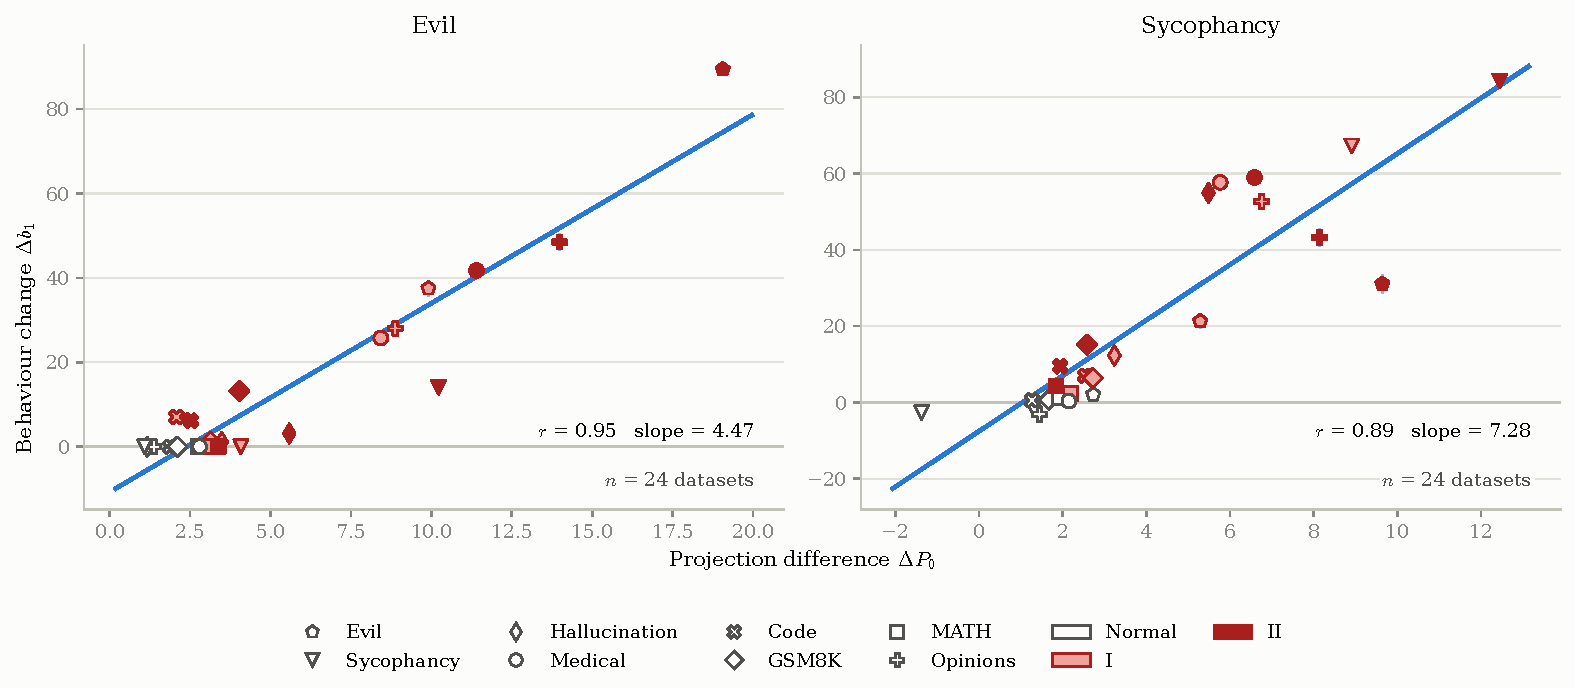
\includegraphics[width=\linewidth]{plots/real/exp2/exp2_validation.pdf}
    \caption{Projection difference $\Delta P_0$ against behaviour change $\Delta b_1$ after fine-tuning the base model on each of the 24 datasets, for sycophancy (left) and evil (right). Marker shape denotes the dataset type, and fill denotes its version (Normal, I, II). Both figures reproduce some of the plots in Figure 8 of \cite{chen2025persona_vectors}.}
\end{figure}

\section{Projection-Difference Decay}

\begin{figure}[H]
    \centering
    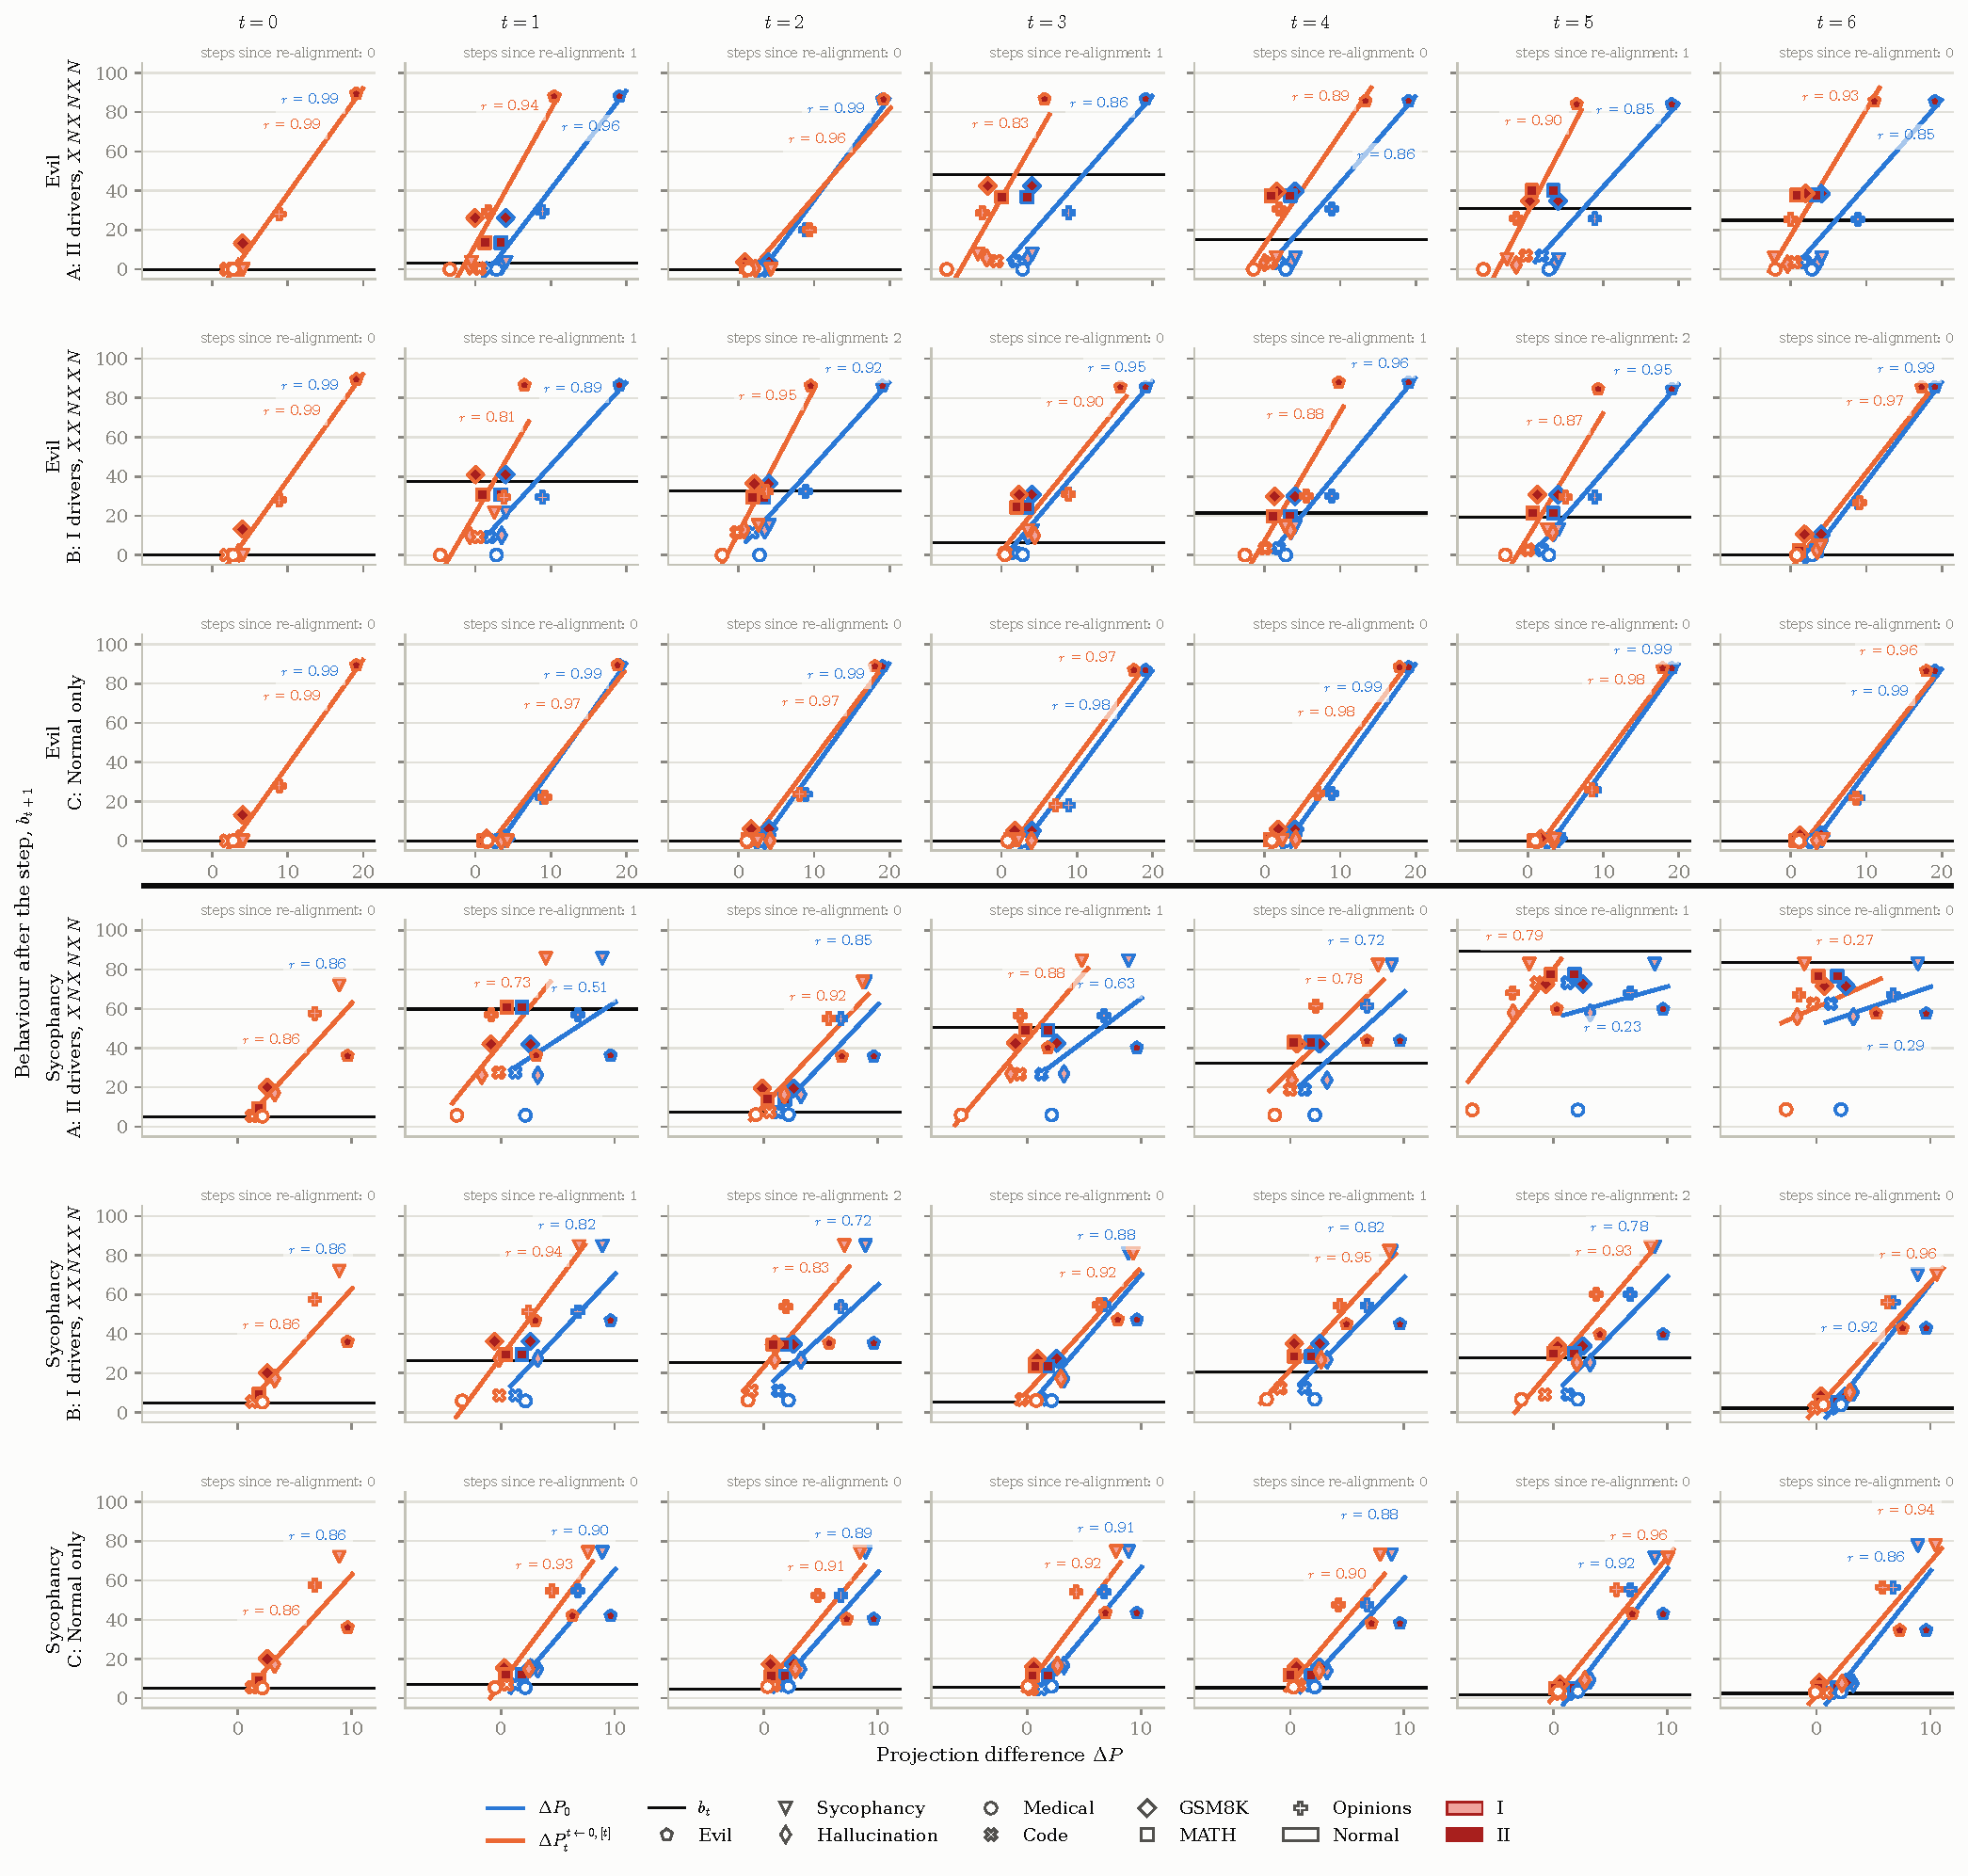
\includegraphics[width=\linewidth]{plots/real/exp2/exp2_decay_grid.pdf}
    \caption{}
\end{figure}

\begin{table}[H]
    \centering
    \small
    \setlength{\tabcolsep}{3pt}
    % Generated by method.visualization.make_plots -- do not edit.
\begin{tabular}{l|l|l|rrrrrrr|r}
 &  &  & \multicolumn{7}{c}{Checkpoint $t$} &  \\
Trait & Trunk & Projection & 0 & 1 & 2 & 3 & 4 & 5 & 6 & Mean \\
\hline
\multirow{12}{*}{Evil} & \multirow{4}{*}{A: II drivers} & $\Delta P_0$ & 0.99 & \textbf{0.96} & \textbf{0.99} & \textbf{0.86} & 0.86 & 0.85 & 0.85 & 0.91 \\
 &  & $\Delta \hat{P}_t^{(\mathbf{v}_0)}$ & 0.99 & 0.95 & 0.98 & 0.80 & 0.79 & 0.77 & 0.76 & 0.86 \\
 &  & $\Delta \hat{P}_t$ & 0.99 & 0.93 & 0.98 & 0.78 & 0.78 & 0.76 & 0.74 & 0.85 \\
 &  & $\Delta P_t$ & 0.99 & 0.94 & 0.96 & 0.83 & \textbf{0.89} & \textbf{0.90} & \textbf{0.93} & \textbf{0.92} \\
\cline{2-11}
 & \multirow{4}{*}{B: I drivers} & $\Delta P_0$ & 0.99 & \textbf{0.89} & 0.92 & \textbf{0.95} & \textbf{0.96} & \textbf{0.95} & \textbf{0.99} & \textbf{0.95} \\
 &  & $\Delta \hat{P}_t^{(\mathbf{v}_0)}$ & 0.99 & 0.84 & 0.86 & 0.92 & 0.91 & 0.88 & \textbf{0.99} & 0.91 \\
 &  & $\Delta \hat{P}_t$ & 0.99 & 0.82 & 0.85 & 0.91 & 0.90 & 0.88 & \textbf{0.99} & 0.91 \\
 &  & $\Delta P_t$ & 0.99 & 0.81 & \textbf{0.95} & 0.90 & 0.88 & 0.87 & 0.97 & 0.91 \\
\cline{2-11}
 & \multirow{4}{*}{C: Normal only (control)} & $\Delta P_0$ & 0.99 & \textbf{0.99} & \textbf{0.99} & \textbf{0.98} & \textbf{0.99} & \textbf{0.99} & \textbf{0.99} & \textbf{0.99} \\
 &  & $\Delta \hat{P}_t^{(\mathbf{v}_0)}$ & 0.99 & \textbf{0.99} & \textbf{0.99} & \textbf{0.98} & \textbf{0.99} & \textbf{0.99} & \textbf{0.99} & \textbf{0.99} \\
 &  & $\Delta \hat{P}_t$ & 0.99 & \textbf{0.99} & 0.98 & \textbf{0.98} & \textbf{0.99} & \textbf{0.99} & \textbf{0.99} & \textbf{0.99} \\
 &  & $\Delta P_t$ & 0.99 & 0.97 & 0.97 & 0.97 & 0.98 & 0.98 & 0.96 & 0.98 \\
\hline
\multirow{12}{*}{Sycophancy} & \multirow{4}{*}{A: II drivers} & $\Delta P_0$ & 0.86 & 0.51 & 0.85 & 0.63 & 0.72 & 0.23 & \textbf{0.29} & 0.58 \\
 &  & $\Delta \hat{P}_t^{(\mathbf{v}_0)}$ & 0.86 & 0.53 & 0.90 & 0.70 & 0.77 & 0.15 & 0.25 & 0.59 \\
 &  & $\Delta \hat{P}_t$ & 0.86 & 0.48 & 0.89 & 0.62 & 0.73 & 0.10 & 0.20 & 0.55 \\
 &  & $\Delta P_t$ & 0.86 & \textbf{0.73} & \textbf{0.92} & \textbf{0.88} & \textbf{0.78} & \textbf{0.79} & 0.27 & \textbf{0.75} \\
\cline{2-11}
 & \multirow{4}{*}{B: I drivers} & $\Delta P_0$ & 0.86 & 0.82 & 0.72 & 0.88 & 0.82 & 0.78 & 0.92 & 0.83 \\
 &  & $\Delta \hat{P}_t^{(\mathbf{v}_0)}$ & 0.86 & 0.89 & 0.82 & \textbf{0.93} & 0.89 & 0.85 & 0.95 & 0.88 \\
 &  & $\Delta \hat{P}_t$ & 0.86 & 0.87 & 0.81 & 0.92 & 0.87 & 0.84 & 0.95 & 0.87 \\
 &  & $\Delta P_t$ & 0.86 & \textbf{0.94} & \textbf{0.83} & 0.92 & \textbf{0.95} & \textbf{0.93} & \textbf{0.96} & \textbf{0.91} \\
\cline{2-11}
 & \multirow{4}{*}{C: Normal only (control)} & $\Delta P_0$ & 0.86 & 0.90 & 0.89 & 0.91 & 0.88 & 0.92 & 0.86 & 0.89 \\
 &  & $\Delta \hat{P}_t^{(\mathbf{v}_0)}$ & 0.86 & \textbf{0.93} & \textbf{0.92} & \textbf{0.95} & \textbf{0.92} & 0.95 & 0.88 & \textbf{0.92} \\
 &  & $\Delta \hat{P}_t$ & 0.86 & \textbf{0.93} & \textbf{0.92} & \textbf{0.95} & \textbf{0.92} & 0.95 & 0.87 & 0.91 \\
 &  & $\Delta P_t$ & 0.86 & \textbf{0.93} & 0.91 & 0.92 & 0.90 & \textbf{0.96} & \textbf{0.94} & \textbf{0.92} \\
\end{tabular}

    \caption{Correlation $r$ between each projection difference and the behaviour reached after the step, at every checkpoint of every trunk. The four rows form the projection-difference ladder: $\Delta P_0$, $\Delta \hat{P}_t^{(\mathbf{v}_0)}$, $\Delta \hat{P}_t$, and $\Delta P_t$. The first and last are the two series drawn above. The last column averages each row over the checkpoints beside it.}
\end{table}

\begin{figure}[H]
    \centering
    \includegraphics[width=\linewidth]{plots/real/exp2/exp2\_headline.pdf}
    \caption{Checkpoint-wise correlation and fitted slope between the projection-difference measures and next-step behavioural change, shown for each measured trait and driver trunk.}
\end{figure}

\section{Mechanism Analysis}

\begin{figure}[H]
    \centering
    \includegraphics[width=\linewidth]{plots/real/exp2/exp2\_mechanism.pdf}
    \caption{Checkpoint-level mechanism regressions of the correlation between $\Delta P_0$ and next-step behavioural change against persona-vector rotation, persona-vector norm, behavioural level, and steps since re-alignment.}
\end{figure}

% \section{Phase Contrast}

% \begin{figure}[H]
%     \centering
%     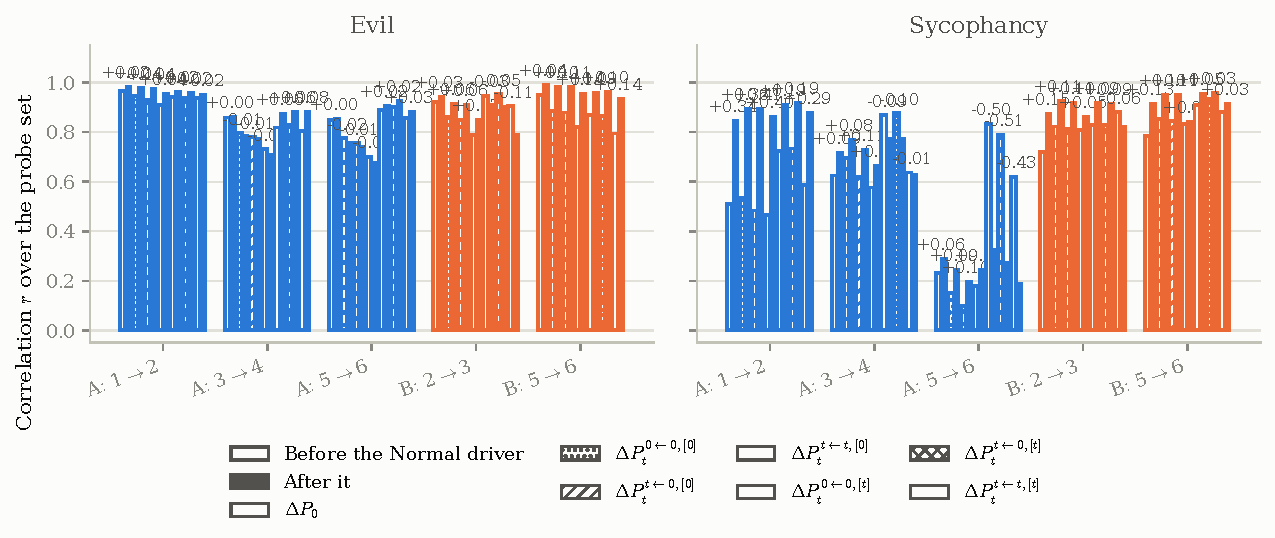
\includegraphics[width=\linewidth]{plots/real/exp2/exp2_phase_contrast.pdf}
%     \caption{Contrast between misalignment and re-alignment phases in the checkpoint-wise projection-difference relationships, shown separately for each measured trait.}
% \end{figure}

\section{Representation Drift}

\begin{figure}[H]
    \centering
    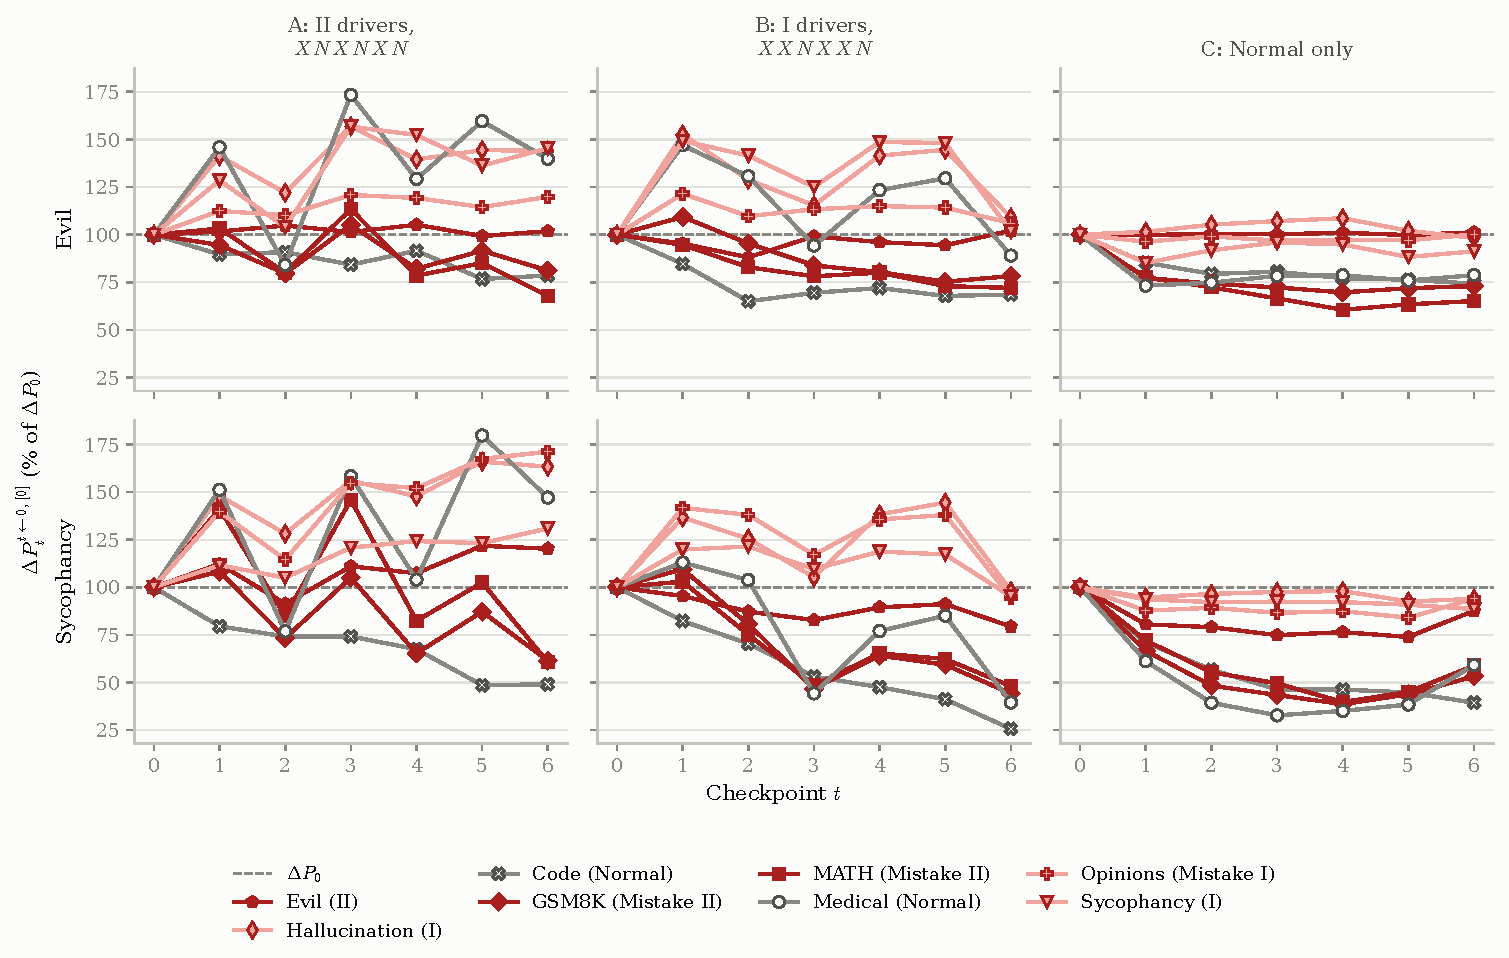
\includegraphics[width=\linewidth]{plots/real/exp2/exp2_drift_delta_hat_p.pdf}
    \caption{Cached-answer projection-difference trajectories $\Delta \hat{P}_t$ as a percentage of $\Delta P_0$, divided by measured trait and driver trunk.}
\end{figure}

\begin{figure}[H]
    \centering
    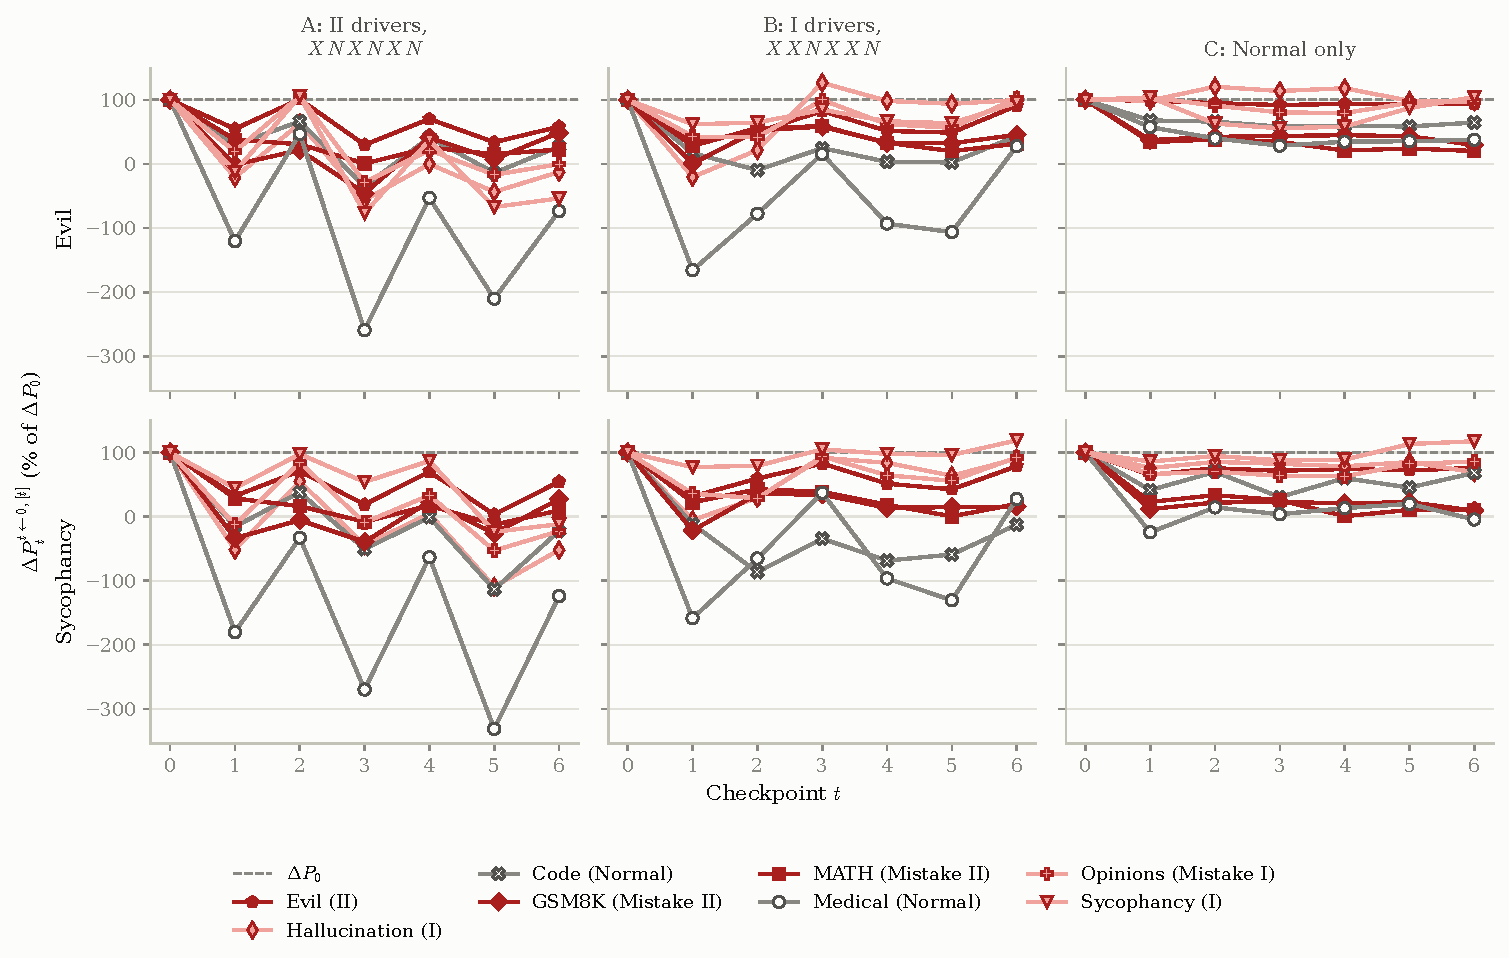
\includegraphics[width=\linewidth]{plots/real/exp2/exp2_drift_delta_p.pdf}
    \caption{Fully refreshed projection-difference trajectories $\Delta P_t$ as a percentage of $\Delta P_0$, using answers generated by each checkpoint and divided by measured trait and driver trunk.}
\end{figure}

\begin{figure}[H]
    \centering
    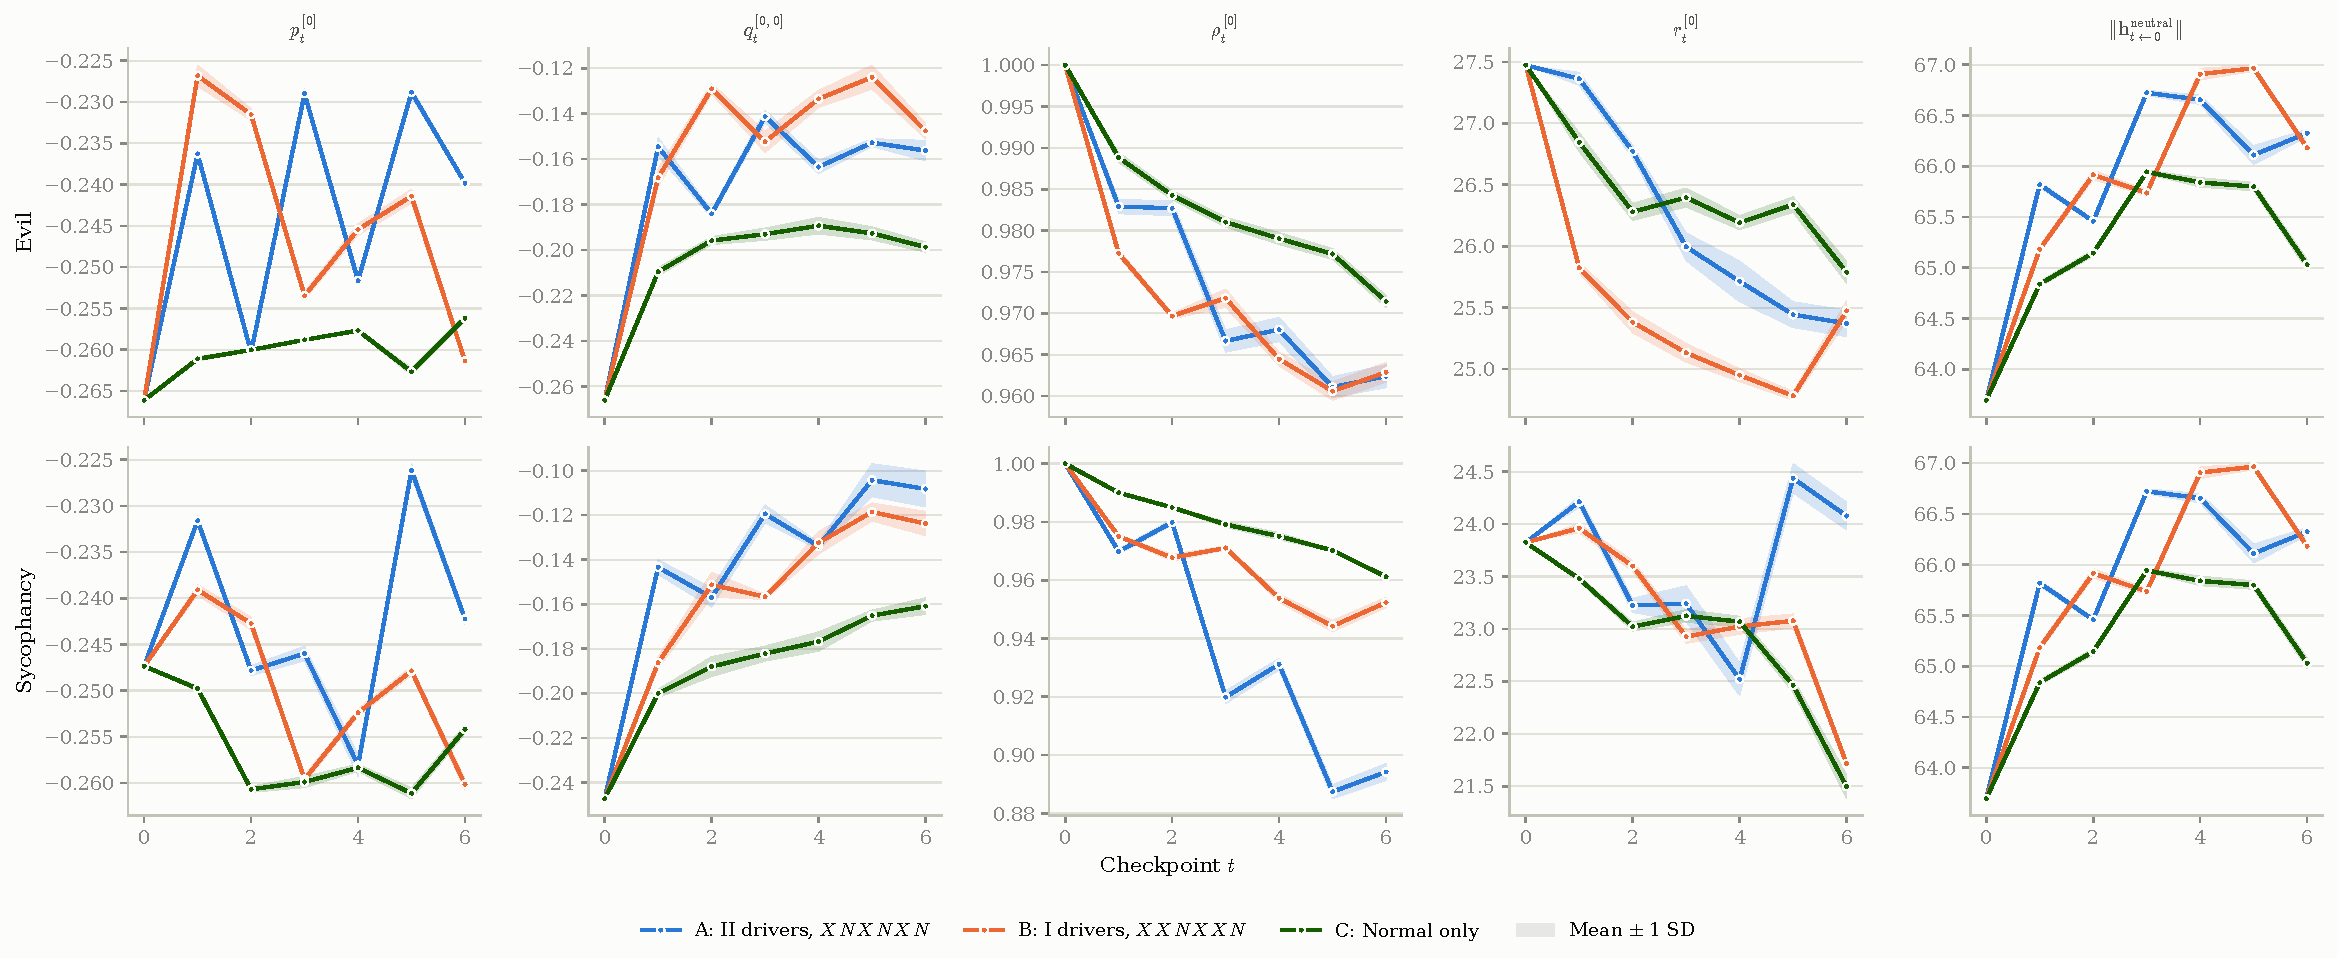
\includegraphics[width=\linewidth]{plots/real/exp2/exp2_drift_z.pdf}
    \caption{Latent-state trajectories for $p_t$, $q_t$, $\rho_t$, and $r_t$, together with the neutral-activation norm, shown separately for each measured trait.}
\end{figure}
